\documentclass{article}
\usepackage{style}

\begin{document}
  \title{FYS1210}
  \author{Robin A. T. Pedersen}
  \maketitle
  \tableofcontents

  \section{Forord}
    Dette dokumentet er hovedsaklig skrevet for meg selv i et forsøk på å tvinge hjernen min til å behandle informasjonen inneholdt i pensum.
Kanskje vil det bli noe andre kan bruke hvis de ikke gidder å lese hele læreboka, eller det kan brukes som oppsummering før eksamen?
\\

Se etter feil og si ifra hvis du gidder.

  \section{Acknowledgments}
    Takk til Dawid Kuleczko som skrev noen av seksjonene,
Kai Morgan Kjølerbakken vår foreleser,
labveileder Ivar Bruvik Martins,
og ElDat.

  \section{Uke 3 - Introduksjon}
    Ledere, isolatorer, halvledere, Ohms lov, serie- og parallellkobling, Kirchoff, superposisjon og Thevenin.

\subsection{Serie- og parallellkobling}
\subsubsection{Seriekobling}
TODO

\subsubsection{Parallellkobling}
TODO


\subsection{Kirchhoff}
\subsubsection{Kirchhoffs lov om strømmer}
TODO



\subsubsection{Kirchhoffs lov om spenninger}
TODO



\subsubsection{Spenningsdeler}
Vi ser på tilfellet med to motstander seriekoblet til et batteri.
\\
\begin{circuitikz} \draw
(0,0) to[battery, l=$V_{batteri}$] (0,4)
      -- (4,4)
      to[R, l=$R_2$] (4,2)
      to[R, l=$R_1$] (4,0)
      -- (0,0)
      ;
\end{circuitikz}
\\
Hva er spenningen $V_1$ over motstanden $R_1$?
$$V_1 = \frac{R_1}{R_1 + R_2} \cdot V_{batteri}$$

Du kan tenke på det som dette:
\\
Hvor stor del av kaka tar $R_1$?
sin rettferdige andel: $\frac{R_1}{R_1 + R_2}$
\\
Hvor mye kake er det egentlig? $V_{batteri}$


\subsection{Superposisjon}
Superposisjonsprinsippet brukes til å finne verdier i kretser med mer enn én spenningskilde.
For å finne spenningen rundt en komponent ser man på bidraget fra én spenningskilde om gangen.
Når bidraget fra alle kildene er funnet, legger man det sammen for å få totalverdien.

\subsubsection{Eksempel}
$V_{S1}=\SI{15}{\volt}$,\qquad
$V_{S2}=\SI{3}{\volt}$,\qquad
$R_1=R_2=R_3=\SI{1}{\kilo\ohm}$



\begin{circuitikz} \draw
(0,0) to[battery, l=$V_{S1}$] (0,4)
      to[R, l=$R_2$] (4,4)
      -- (8,4)
      to[R, l=$R_1$] (8,0)
      -- (0,0)
(4,0) to[battery, l=$V_{S2}$] (4,2)
      to[R, l=$R_3$] (4,4)
      ;
\end{circuitikz}
\\
I denne kretsen er det to spenningskilder som begge bidrar til å
skape spenning $V_1$ rundt motstanden $R_1$.



\begin{circuitikz} \draw
(0,0) to[battery, l=$V_{S1}$] (0,4)
      to[R, l=$R_2$] (4,4)
      -- (8,4)
      to[R, l=$R_1$] (8,0)
      -- (0,0)
(4,0) -- (4,2)
      to[R, l=$R_3$] (4,4)
      ;
\end{circuitikz}
\\
Vi later som den ene spenningskilden $V_{S2}$ ikke eksisterer
og regner ut bidraget fra $V_{S1}$.



\begin{circuitikz} \draw
(0,0) to[battery, l=$V_{S1}$] (0,4)
      to[R, l=$R_2$] (4,4)
      to[R, l=$R_{EQ}$] (4,0)
      -- (0,0)
      ;
\end{circuitikz}
\\
Motstandene $R_1$ og $R_3$ danner en parallellkobling som vi kan
betrakte som én motstand $R_{EQ}$.
Siden $R_1$ og $R_3$ er parallellkoblet får man
$R_3$ via den \emph{inverse}.
$$\frac{1}{R_{EQ}} = \frac{1}{R_1} + \frac{1}{R_3}$$
Eller, siden det bare er to motstander, via forenklingen.
$$R_{EQ} = \frac{R_1 \cdot R_3}{R_1 + R_3} = \frac{1\cdot 1}{1+1}=\frac{1}{2}$$
%TODO: enheter


  \section{Uke 4 - Fysikalsk elektronikk}
    Kap.  7, s.203-217 \\
Kap.  9, s.247-279 \\
Kap. 12, s.364-382 \\
Kap. 13, s.389-413 \\
Kap. 15, s.462-500 \\
Kap. 16, s.510-528

\subsection{Thevenins Teorem}
\subsubsection{Last-analyse}
Thevenins teorem er en regneteknikk hvor du kan betrakte noe komplisert som noe enkelt.
Det brukes som regel for å regne på forksjellig last uten å måtte regne ut hele kretsen på nytt.

\begin{circuitikz} \draw
(0,0) -- (0,4)
      node [right=3em,below=3em,anchor=west]
           {\large{\textsc{Komplisert krets}}}
      -- (6,4)
      -- (6,0)
      -- (0,0)
(6,3) to[short, -o] (7,3)
      to[voltmeter] (7,1)
      to[short, o-] (6,1)
      ;
\draw[dashed]
(7,3) -- (8,3)
      to[R, label=$R_L$] (8,1)
      -- (7,1)
      ;
\end{circuitikz}
\\
Alle topolede, lineære nettverk (krets)...
\\\\

\begin{circuitikz} \draw
(0,0) -- (0,4)
      -- (6,4)
      -- (6,0)
      -- (0,0)
(6,3) to[short, -o] (7,3)
      to[voltmeter] (7,1)
      to[short, o-] (6,1)
      -- (1,1)
      to[battery] (1,3)
      node[right=1em,below=2.5em,anchor=west]{$V_{TH}$}
      to[R, label=$R_{TH}$] (6,3)
      ;
\draw[dashed]
(7,3) -- (8,3)
      to[R, label=$R_L$] (8,1)
      -- (7,1)
      ;
\end{circuitikz}
\\
...kan erstattes med en spenningskilde $V_{TH}$ og en motstand $R_{TH}$.
\\\\
$V_{TH}$=Spenningen over polene uten last.\\
$R_{TH}$=Motstand over polene når alle spenningskilder er kortsluttet og alle strømmer brutt.



\subsubsection{Eksempel}
\begin{circuitikz} \draw{}
(0,1) -- (0,0) node[ground]{}
(0,0) to[battery, label=$V_S$] (0,4)
      to[R, label=$R_1$] (4,4)
      to[R, label=$R_2$] (4,2)
      to[R, label=$R_3$] (4,0)
      node[ground]{}
(4,2) -- (8,2)
      to[R, label=$R_L$] (8,0)
      node[ground]{}
      ;
\end{circuitikz}
\\
Denne kretsen kan skrives om til å ligne på beskrivelsen av Thevenin ovenfor.
\\

\begin{circuitikz} \draw{}
(1,1) to[battery, label=$V_S$] (1,3)
      to[R, label=$R_1$] (3,3)
      to[R, label=$R_2$] (5,3)
      to[R, label=$R_3$] (5,1)
      -- (1,1)
(5,3) to[short, -o] (7,3)
(5,1) to[short, -o] (7,1)
(0,0) -- (0,4)
      -- (6,4)
      -- (6,0)
      -- (0,0)
      ;
\draw[dashed]
(7,3) -- (8,3)
      to[R, label=$R_L$] (8,1)
      -- (7,1)
      ;
\end{circuitikz}
\\

Vi regner ut $V_{TH}$:\\
Spenning målt over polene uten last,
tilsvarer å måle spenning rundt $R_3$.\\
(Husk at $R_1$ og $R_2$ står i serie)
$$V_{TH} = V_3 = \frac{R3}{(R_1 + R_2) + R_3} \cdot V_S$$
\\

Vi regner ut $R_{TH}$:\\
Motstand over polene når spenningskilder er kortsluttet,
blir som å betrakte kretsen som en parallellkobling.
$$R_{TH} = \frac{(R_1 + R_2)R_3}{(R_1 + R_2) + R_3}$$


\subsubsection{Nortons Teorem}
TODO


\subsection{Spenningskilder - Batterier}
\subsubsection{Virkemåte}
TODO

\subsubsection{Maksimal effektoverføring}
TODO


\subsection{Fysikalsk elektronikk}
Etter Niels Bohrr atommodell ligger elektroner i skall rundt atomkjernen.
Disse skallene kalles bånd.

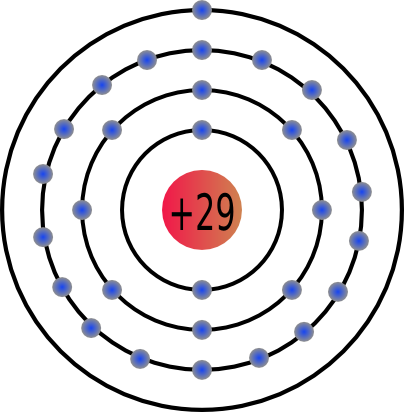
\includegraphics[width=0.25\textwidth]{./img/bohr-Cu}
\\
Kobberatom med 29 protoner og 29 elektroner.\\
Skall 1: 2 elektroner \\
Skall 2: 8 elektroner \\
Skall 3: 18 elektroner \\
Skall 4: 1 elektron
\\
Det ytterste elektronet har en svakere binding til kjernen.

TODO


\subsection{Doping}
TODO


\subsection{Vekselstrøm}
TODO


\subsection{DC-Offset}
TODO


\subsection{Pulser}
TODO


  \section{Uke 5 - Kondensatorer}
    Kap. 12, s.364-382 \\
Kap. 13, s.389-413 \\
Kap. 15, s.462-500 \\
Kap. 16, s.510-528 \\
Kap. 17, s.533-564 \\
Kap. 18, s.574-605

\subsection{Kondensatorer}
\subsubsection{Beskrivelse}
En kondensator (engelsk: capasitor)
er en av de mest fundamentale kompenentene vi bruker.
Dens funksjon er å lagre elektrisk ladning.
De brukes bl.a. til lokal energilagring (som et lite batteri),
dempe brå forandring av spenning (for å beskytte sårbare komponenter)
og signalfiltrering.



\subsubsection{Virkemåte og symbol}
En kondensator består av to ledende plater
med et isolerende materiale (et dielektrisk) i mellom.
\\
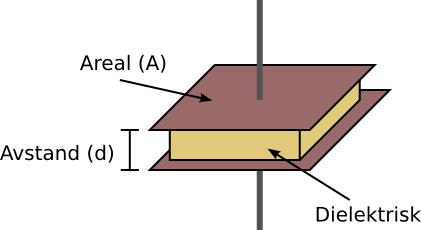
\includegraphics[width=0.5\textwidth]{./img/kondensator-basic}
\\\\
\emph{Symbolet} for en kondensator gjenspeiler oppbygningen.
\\
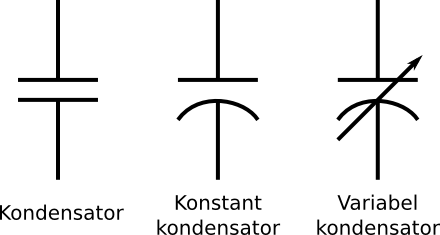
\includegraphics[width=0.5\textwidth]{./img/kondensator-symboler}
\\
\paragraph{Spenning} \mbox{} \\
Når en kondensator kobles til en spenningskilde
vil det gå strøm gjennom kretsen.
Elektronene strømmer \emph{mot} den ene siden av kondensatoren,
og \emph{fra} den andre siden.
\\
Men strømmen blir blokkert av dielektrikumet
og går ikke gjennom kondensatoren.
Istedenfor samler elektronene seg på den ene siden,
og det blir en mangel på elektroner på andre siden.
\\
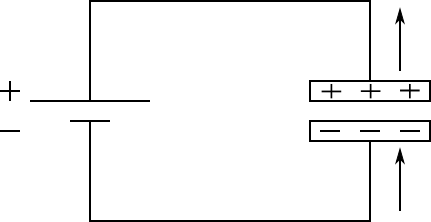
\includegraphics[width=0.5\textwidth]{./img/kondensator-ladning}
\\
Man kan tenke på det som om det går to strømmer.
En fra negativ pol til kondensatoren.
Og en fra kondensatoren mot positiv pol.
\\\\
Nå er det negative ladninger på den ene siden,
og positive på den andre.
Det vil si at vi har en spenning over kondensatoren.



\subsubsection{Formler og enheter}
Kapasitet(ladning), kapasitet(areal), serie, parallell \\
TODO


\subsection{Kondensatorer i kretser}
\subsubsection{DC-kretser}
Impossible for current [...] across cap (in DC?) \\
TODO

\subsubsection{AC-kretser}
Faseforskyvning \\
Reaktanse \\
Decoupling caps \\
TODO

\subsubsection{RC-kretser}
Impedans \\
TODO


\subsection{Frekvensfilter}
\paragraph{Lavpass} \mbox{} \\
TODO



\paragraph{Høypass} \mbox{} \\
TODO



\paragraph{Eksempel} \mbox{} \\
TODO


\subsection{Dioder}
TODO


  \section{Uke 6 - Dioder}
    Kap. 17, s.533-564
Kap. 18, s.574-605

\subsection{Kovalente bindinger}
\subsubsection{Diamantstruktur}
Vi vet allerede at halvledere har 4 elektroner i valensbåndet.
Etter oktettregelen ønsker disse atomene
å fullføre sitt ytterste skall med 8 elektroner.
For å oppnå dette, danner de kovalente bindinger (elektronparbininger)
med andre atomer.
\\
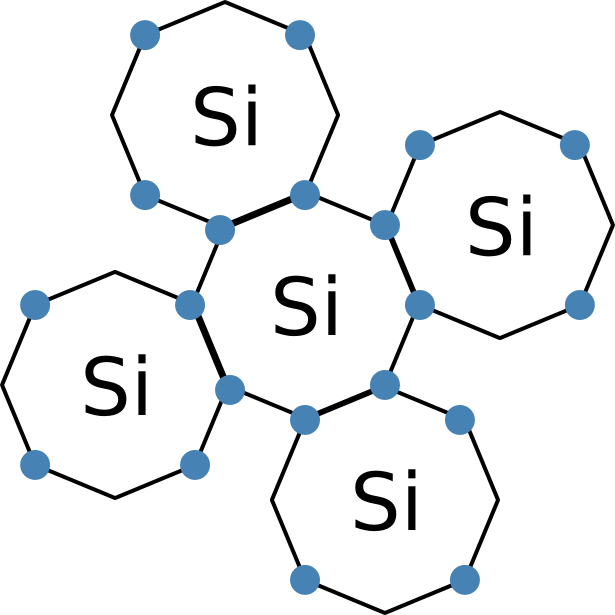
\includegraphics[width=0.5\textwidth]{./img/krystall.png}
\\
Silisiumatmoer danner en krystallstruktur.

\subsubsection{Ledning i rene halvledere}
Ved tilført energi (varme eller lys) kan elektronene løsrives
fra valensbåndet og bevege seg fritt i ledningsbåndet.
\\
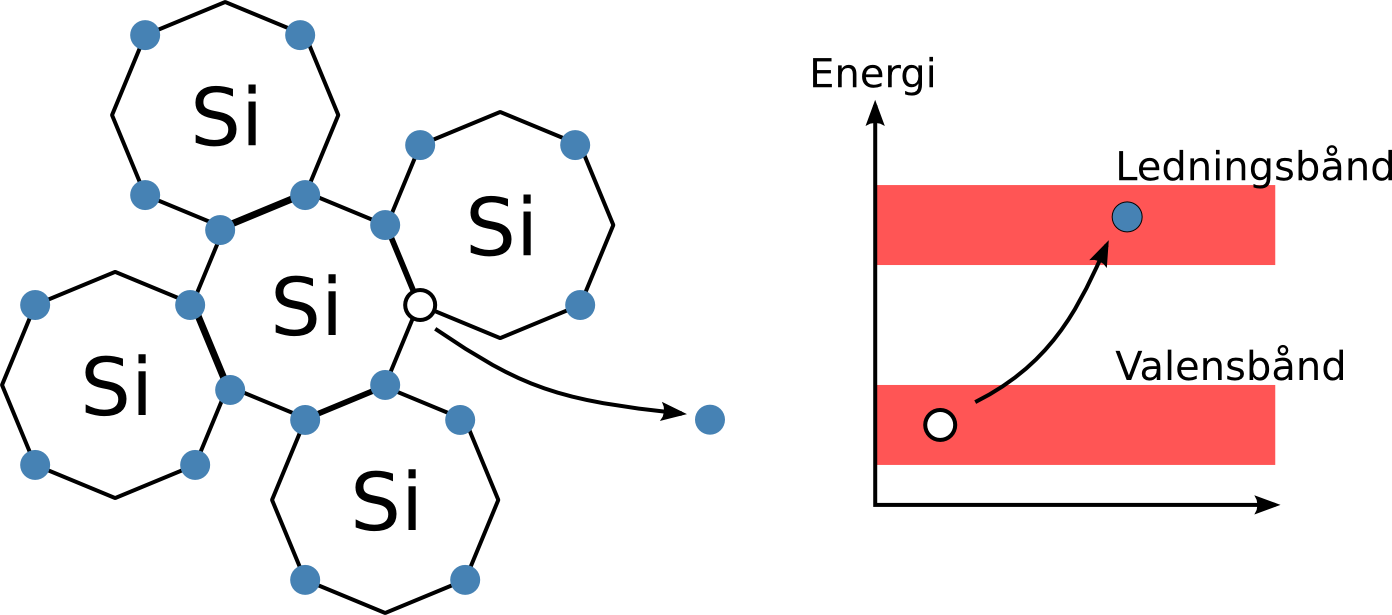
\includegraphics[width=\textwidth]{./img/krystall-ledning.png}
\\
Når elektroner faller tilbake igjen, ned i disse hullene,
kalles des rekombinasjon.


\subsection{Doping}
Hvordan doping fungerer er beskrevet i tidligere seksjoner.

\subsubsection{Pentavalent}
Pentavalente grunnstoffer (n-type) har 5 valenselektroner.
Dette gir et overflødig elektron som er svakt bundet.
Husk, stoffet er fremdeles nøytralt!
I denne type doping er elektronene majoritetsbærere.
\\\\
Eksempel:\\
P - fosfor\\
As - Arsenikk\\
Sb - Antimov\\
Bi - Bismut

\subsubsection{Trivalent}
Trivalente grunnstoffer (p-type) har 3 valenselektroner.
Vi får et hull blandt kovalentbindingene.
Elektroner er minoritetsbærere.
\\\\
Eksempel:\\
B - Bor\\
Al - Aluminium\\
Ga - Gallium\\
In - Indium


\subsection{PN-Junction}
Forklaring m/illustrasjon
Diffusjon
Forward bias
Reverse bias
TODO

\subsection{Dioder}
Forklaring, symbol etc
Ideell karakteristikk
Bulk resistans
Diode identifikasjon
TODO

  \section{Uke 7 - Bipolar Junction Transistorer (BJT)}
    Kap. 19, s. 617-652
+ notater på nett

\subsection{Oppbygning}
En bipolar junction transistor bruker både elektron- og hullstrøm,
og har 2 \emph{junctions} mellom ulikt dopede halvledere.
BJTer kommer i 2 typer, NPN og PNP. Vi skal se på den første av dem.

\paragraph{Collector, Base og Emittor} \mbox{} \\
En BJT består av 3 deler: collector, base og emittor.
Disse er bygget opp av tre dopede halvleder materialer, n-type og p-type.
Mellom disse regionene er pn-overganger akkurat som i dioder. \\\\
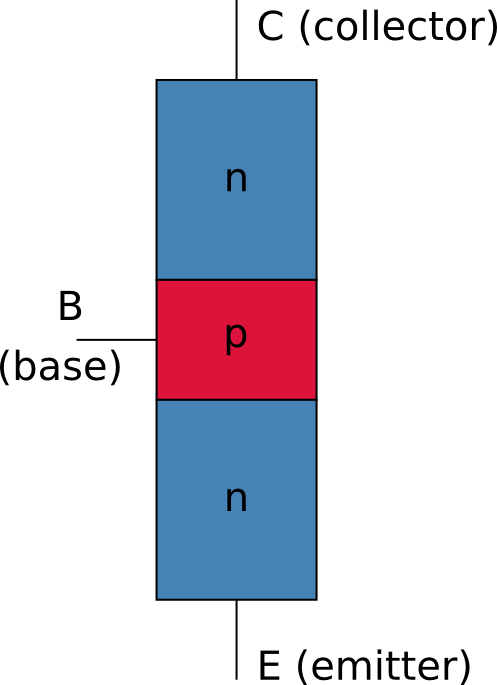
\includegraphics[width=0.5\textwidth]{./img/npn}
\\\\
Symbolet for BJTer ser slik ut for npn \\\\
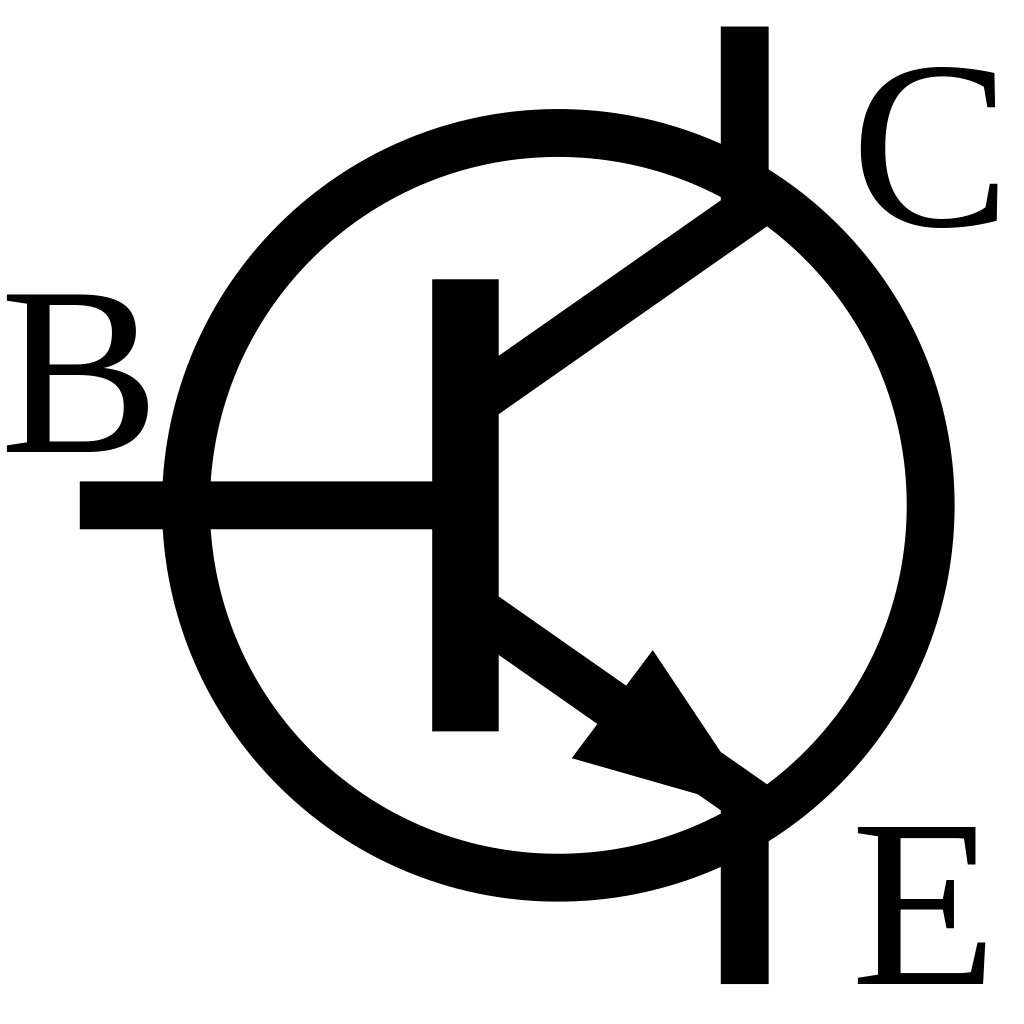
\includegraphics[width=0.25\textwidth]{./img/npn-symbol} \\
Hvor den lille pilen peker mot det n-dopede materialet.
\\
Tilsvarende for pnp \\\\
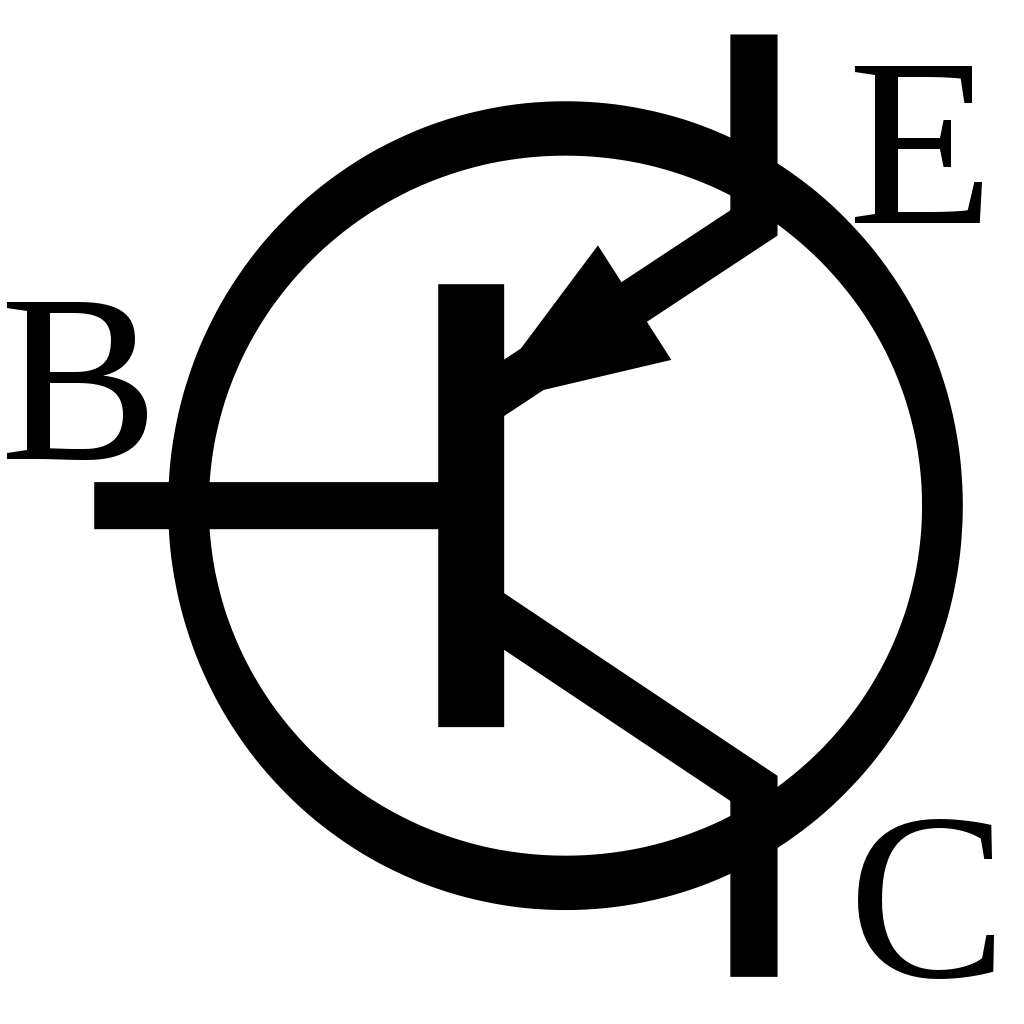
\includegraphics[width=0.25\textwidth]{./img/pnp-symbol}


\paragraph{Fysisk struktur} \mbox{} \\
I virkeligheten er en BJT bygget opp lag på lag med en isolator rundt.
\\\\
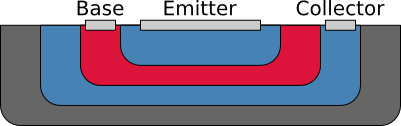
\includegraphics{./img/npn-real}


\subsection{Virkemåte}
  \subsubsection{Operasjonsmodi}
    Siden NPN-transistoren består av 2 PN-overganger,
kan man anse det som to dioder koblet sammen.
\\\\
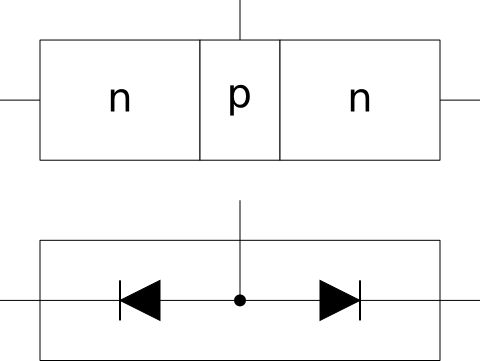
\includegraphics[width=0.5\textwidth]{./img/npn-bias}
\\\\
Disse diodene kan kjøres i forskjellig bias (forward, reverse).
Avhengig av forholdet mellom spenningen
ved diodens collector, base og emitter, fungerer transistoren forskjellig.

De forskjellige kombinasjonene utgjør transistorens operasjonsmodi.
\\\\
\begin{tabular}{ l | c | r}
Base-Emitter & Base-Collector & Operasjonsmodi \\ \hline
Reverse & Reverse & Cutoff \\
Forward & Reverse & Aktiv \\
Forward & Forward & Metning \\
\end{tabular}

  \subsubsection{Cutoff modus}
    Både base-emitter junction og collector-base junction
er i reverse bias.
Vi vet fra hvordan dioder fungerer at sperresjiktet
mellom de dopede materialene vokser.
I cutoff modus fungerer transistoren som en åpen krets,
ingen strøm passerer gjennom.
\\\\
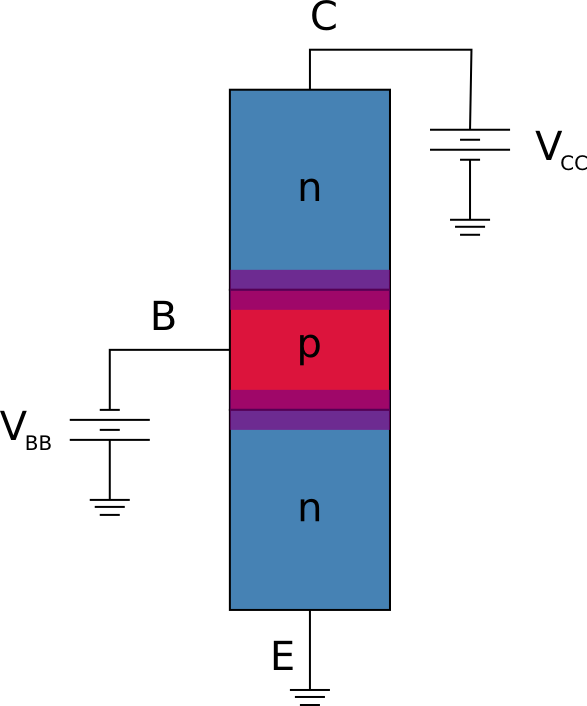
\includegraphics[width=0.5\textwidth]{./img/npn-cutoff}

  \subsubsection{Metning}
    Når spenningen ved basen er større enn ved collector,
fungerer transistoren som en kortslutning.
Strøm går fra emitter til collector.
\\\\
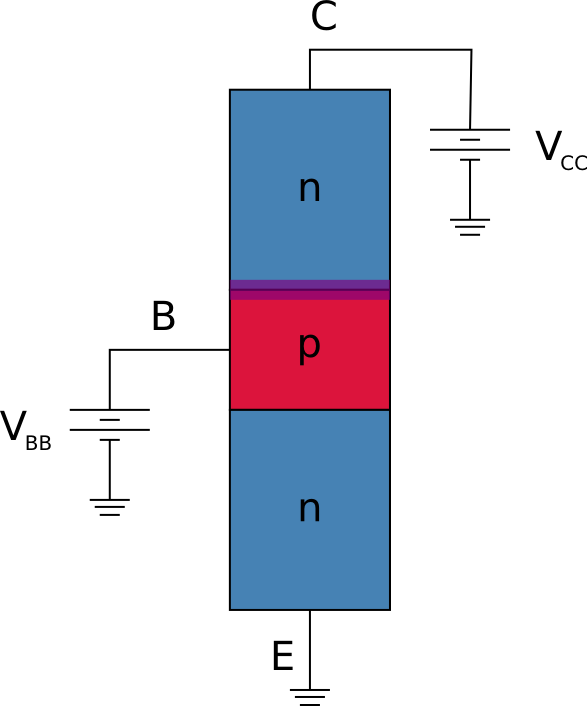
\includegraphics[width=0.5\textwidth]{./img/npn-metning}

  \subsubsection{Aktiv}
    Aktiv modus ser lik ut som ved metning, men med en forskjell.
Spenningen ved collector er større enn ved base.
$$V_C > V_B > V_E$$
I aktiv modus er strømmen fra emitter til collector
proporsjonal med strømmen til base.

  \subsubsection{Modi-kvadrant}
    En annen måte å illustrere transistorens modi på
er ved forholdet mellom spenningene.
\\\\
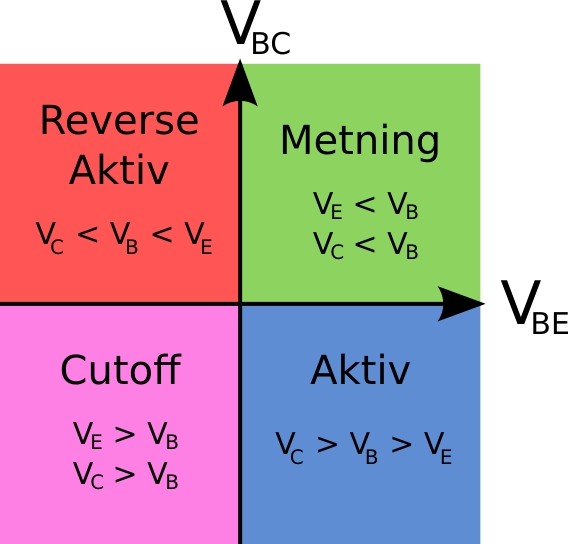
\includegraphics[width=0.5\textwidth]{./img/modi-kvadrant}
\\\\
$V_C = $ spenning fra collector til jord. \\
$V_E = $ spenning fra emitter til jord. \\
$V_B = $ spenning fra base til jord. \\
$V_{BC} = $ spenning fra base til collector. \\
$V_{BE} = $ spenning fra base til emitter. \\


\subsection{Karakteristikk}
  \subsubsection{Strøm}
    TODO

  \subsubsection{Virkeområde}
    TODO


  \section{Uke 8 - Transistorforsterkere og småsignalmodeller}
    Kap. 20, s 662 -695

\subsection{Universal Bias}
Her har det vært mye uklarheter.


Vi er blitt fortalt at det norske ordet
for universal bias er spenningsfordeler.
Etter å ha sett på flere kilder ser det ut til at
spenningsfordeling er noe som skjer, og må tas hensyn til,
under universal bias stabilization.

Formålet med universal bias stabilization, er å få et
stabilt Q-punkt (forklart straks).
Dette er bra for å få en gjevn $I_C$ uavhengig av $\beta$.

\subsubsection{Lastlinje}
Lastlinjen viser alle \emph{mulige} kombinasjoner av $I_C$ og $V_{CE}$.

For å ta hensyn til temperaturforandringer og andre forstyrrelser,
velger vi et punkt midt på denne linja.
\\\\
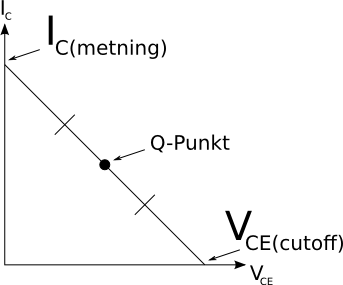
\includegraphics[width=0.5\textwidth]{./img/lastlinje}
\\\\
$$I_{C(metning)} = \frac{V_{CC}}{R_C}$$
$$V_{CE(cutoff)} = V_{cc}$$
Man bruker dette når man velger hvor store motstandere man vil ha.
$$R_C = \frac{V_{CE}}{I_C}$$



\subsection{Småsignalmodellen}
Småsignalmodellen brukes til å se hvordan en transistor
reagerer på små signaler ved å dele transistoren i to deler.
En dynamisk motstand $r_\pi$ mellom base-emitter.
Og en strømgenerator mellom collector-emitter.
Strømgeneratorens strøm bestemmes av transistorens
transkonduktans $g_m$ (steilhet).
\\\\
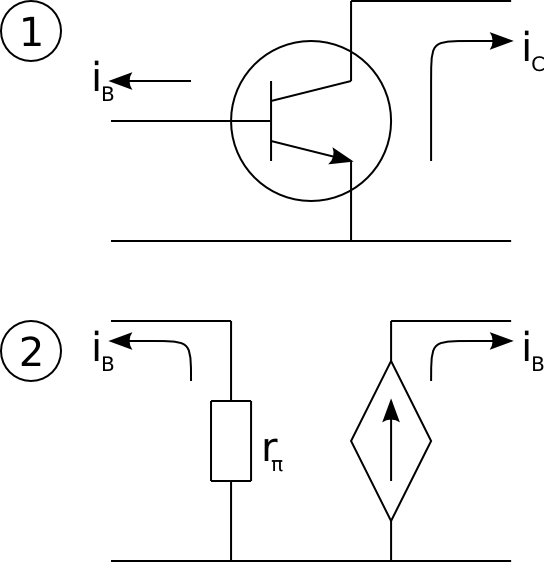
\includegraphics[width=0.5\textwidth]{./img/smasignal}
\\\\
$$i_C = \beta \cdot i_B$$
$$i_C = g_m \cdot V_{BE}$$

\subsubsection{Steilhet}
Transkonduktans?
TODO

\subsubsection{Dynamisk inngangsresistans}
TODO


\subsection{Spenningsforsterkning}
TODO


  \section{Uke 9 - Effektforsterkere og FET}
    Kap. 21, s. 704 -740
Kompendium om digitale kretser.

\subsection{Kort repetisjon av uke8}
  \subsubsection{Forsterker}
    \paragraph{Med avkoblet emitter} \mbox{} \\
\begin{circuitikz} \draw
(4,3) node[npn] (npn) {}
      (npn.base) node[anchor=east] {}
      (npn.collector) node[anchor=south] {}
      (npn.emitter) node[anchor=north] {}

(0,3) node[label=$in$] {}
      to[C, l=$C_1$] (2,3)
      to[R, l=$R_1$] (2,6)
      -- (4,6)
      to[short, -o, l=$V_{CC}$] (4,7)
(4,6) to[R, l=$R_C$] (npn.collector)

(2,3) -- (npn.base)
(npn.emitter) to[R, l=$R_E$] (4,0)
      -- (1,0)
      node[ground] {}
(2,3) to[R, l=$R_2$] (2,0)

(4,2) -- (6,2)
      to[C, l=$C_3$] (6,0)
      -- (4,0)

(4,4) -- (5,4)
      to[C, l=$C_2$] (7,4)
      to[short, -o, l=$out$] (8,4)
      ;
\end{circuitikz}
\\
I denne kretsen er forsterkningen gitt ved
$$A_V = -g_m \cdot R_C$$
\\
Eventuelt, hvis du har en last på output
$$A_V = -gm \cdot (R_C || R_L)$$
\\
Hvor vi \emph{husker} at
$$g_m = \frac{I_C}{V_T}$$



\paragraph{Uten avkoblet emitter} \mbox{} \\
Uten avkoblet emitter kan du ta vekk kondensatorene på høyre side av kretsen.
Da blir forsterkningen (uten last)
$$A_V = -\frac{R_C}{R_E}$$



\paragraph{Småsignaler} \mbox{} \\
Kretsen ovenfor sett ifra småsignalmodellen gir
\\
\begin{circuitikz} \draw
(1,0) to[R, l=$R_{B1}$] (1,4)
(3,0) to[R, l=$R_{B1}$] (3,4)
(6,0) to[R, l=$R_E$] (6,2)
      -- (5,2)
      to[R, l=$r_\pi$] (5,4)
      node[label=$B$] {}
      to[short, -o] (0,4)
      node[label=$V_{inn}$] {}
(6,2) -- (7,2)
      to[american controlled current source] (7,4)
      node[label=$C$] {}
      to[short, -o] (9,4)
      node[label=$V_{ut}$] {}
(8,4) to[R, l=$R_C$] (8,0)
(9,0) to[short, o-o] (0,0)
      ;
\end{circuitikz}
\\
Motstanden som signalet ser inn mot kretsen er
$$R_{inn} = R_{B1} || R_{B2} || r_{inn}$$
\\
Hvor $r_{inn}$ er motstanden etter de 2 parallell-motstandene.
$$r_{inn} = r_\pi + (\beta + 1)R_E$$

  \subsubsection{Emitterfølger}
    Emitterfølger er når vi måler $V_{ut}$ fra emitter istedenfor collector.
I motsetning til den forige kretsen, blir det ingen invertering av signalet.
Det blir heller ingen spenningsforsterkning, men stor effektforsterkning.
\\\\
Strømforsterkningen er gitt ved
$$A_i = \frac{i_e}{i_b}
= \frac{i_b(\beta +1)}{i_b} = \beta + 1$$
\\
Effektforsterkningen er gitt ved
$$A_P = A_V \cdot A_i
\cong 0.99 \cdot (\beta + 1)$$
$$A_P \approx \beta$$


\subsection{Effektforsterkere}
  \paragraph{Klassifisering av forsterkere} \mbox{} \\
Forksjellige parametre definerer egenskapene til en forsterker.
Avhengig av hvilken karakteristikk man ser på kan forsterkerne klassifiseres.
\\
\begin{itemize}
\item Lav og høy frekvens
\item Avstemt og uavstemt
\item Smalbånd og bredbånd
\end{itemize}

I de følgende seksjonene skal vi se på effektforsterkere og hvordan de deles inn
etter hvordan transistorens arbeidspunkt er plassert på lastlinja.
\\
Effektforsterkere har en virkningsgrad som sier noe om effekten ut
i forhold til effekten inn.
$$\eta = \frac{P_L}{P_{CC}} $$
Hvor \\
 $P_L$ = Effekt avgitt fra lasten og \\
$P_{CC}$ = Effekt tilført fra CC.

\subsubsection{Klasse A}
Arbeidspunktet ligger midt på lastlinja.
Altså i det aktive området.
\\
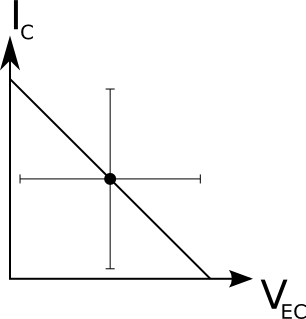
\includegraphics[width=0.5\textwidth]{./img/typeALastlinje}
\\\\
Effektforsterker klasse A (emitterfølger)
\\
\begin{circuitikz} \draw
(4,2) node[npn] (npn) {}
      (npn.base) node[anchor=east] {}
      (npn.collector) node[anchor=south] {}
      (npn.emitter) node[anchor=north] {}

(0,2) node[label=$V_{inn}$] {}
      to[C, o-] (2,2)
      -- (npn.base)
(2,2) to[R, l=$R_1$] (2,4)
      -- (4,4)
      -- (npn.collector)
(2,2) to[R, l=$R_2$] (2,-1)
(npn.emitter) to[R, l=$R_E$] (4,-1)
(4,1) to[short, -o] (6,1)
      node[label=$V_{ut}$] {}
(4,-1) -- (0,-1)
      node[ground] {}
      ;
\end{circuitikz}
\\\\
TypeA effektforsterkere har lav virkningsgrad. f.eks $\eta = 25\%$.
Denne klassen trekker strøm når det ikke er tilført signal.


\subsubsection{Klasse B}
Arbeidsområdet er på grensa mellom aktiv og cutoff.
\\
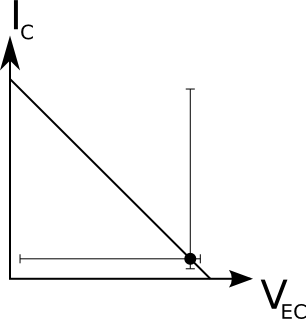
\includegraphics[width=0.5\textwidth]{./img/typeBLastlinje}
\\
I en klasse B emitterfølger blir det en effektforsterkning som kun
virker på halvperioder.
Output signalet tar ikke med negativt input signal.
\\\\
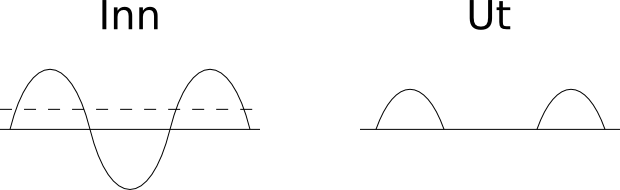
\includegraphics[width=0.67\textwidth]{./img/klasseBSignal}
\\\\
En slik forsterker ser slik ut
\\
\begin{circuitikz} \draw
(4,3) node[npn] (npn) {}
      (npn.base) node[anchor=east] {}
      (npn.collector) node[anchor=south] {}
      (npn.emitter) node[anchor=north] {}

(0,0) node[ground] {}
      to[vsourcesin, l=$V_{inn}$] (0,3)
      -- (npn.base)
(npn.collector) to[short, -o, l=$V_{CC}$] (4,4)
(npn.emitter) -- (4,2)
      to[R, l=$R_E$] (4,0)
      node[ground] {}
(4,2) to[short, -o, l=$V_{ut}$] (5,2)
      ;
\end{circuitikz}
\\\\
Det finnes også \emph{Push-Pull} klasse B forsterkere.
De bruker både npn og pnp og fanger både positive og negative signaler, men
med \emph{crossover} forvrengning.
\\\\
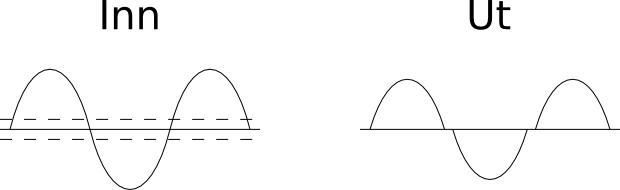
\includegraphics[width=0.67\textwidth]{./img/crossover}


\subsubsection{Klasse AB}
TODO


\subsubsection{Klasse C}
TODO


\subsubsection{Klasse D}
TODO



\subsection{Field Effekt Transistor}
  FET, field effekt transistor, er en type transistor.
En FET kalles en \emph{unipolar} komponent fordi de har én type bærere.
Ladningstransporten skjer ved majoritetsbærere.

Fordeler:
\begin{itemize}
\item Spenningsregulert: Kan anses som en spenningskontrollert strømkilde.
\item Veldig stor inngangsmotstand. Som gjør den energieffektiv.
\end{itemize}

Ulemper:
\begin{itemize}
\item Lav transkonduktans. Som gir liten forsterkning.
\end{itemize}



\subsubsection{To typer}
Field effekt transistorer kommer i 2 typer
\\
\paragraph{JFET: Junction Field Effekt Transistor} \mbox{} \\
JFET er den første typen FET som ble laget.
De deles igjen i to typer, n-channel og p-channel, avhengig av hva slags doping
som er brukt på den innerste halvlederen.
\\
\paragraph{MOSFET: Metall Oksyd Semiconductor FET} \mbox{} \\
MOSFET er en nyere teknologi enn JFET.
Kommer også som n-channel eller p-channel, men kommer i tillegg som en av:\\
E-MOSFET - Enhancement mode MOSFET (er på med tilstrekkelig spenning på gate) \\
D-MOSFET - Depletion mode MOSFET (er på uten spenning på gate)



\subsubsection{JFET}
TODO

\subsubsection{MOSFET}
TODO

\subsubsection{CMOS}
TODO


\subsection{Logic Gates}
  Binære systemer \\
Boolsk algebra \\
Bygges opp av 3 porter \\
Sannhetstabell (truth table) \\
TODO


  \section{Uke 10 - Digitale kretsfamilier}
    Eget kompendium om digitale kretser.

\subsection{Kretsfamilier (Logic families)}
  Kretsfamilier refererer til forksjellige teknikker som brukes til å
implementere logikk.
\\\\
Det finnes mange av disse: RTL, DCTL, RCTL, DTL, CTDL, HTL, ECL, PECL, LVPECL,
GTL, TTL, PMOS, NMOS, HMOS, CMOS, BiCMOS, IIl.
\\\\
Heldigvis skal vi bare se på noen få av dem.



\paragraph{Bipolare komponenter (BJT)} \mbox{} \\
Dioder-vakuumrør ble brukt i de første elektroniske datamaskinene
på 1940-tallet.
\\\\
DTL, diode-transistor logikk, ble først brukt på 50-tallet når man byttet ut
vakuumrørene med transistorer.
\\\\
ECL, emitter-coupled logikk, er raske integrerte kretser som bruker for mye
energi. De ble brukt mellom 1970-1990, men kan også bli brukt i dag.
\\\\
TTL, transistor-transistor logikk, er mye brukt i integrerte kretser.
Etter oppfinnelsen på 60-tallet er de fremdeles i bruk i dag.



\paragraph{Unipolare komponenter (FET)} \mbox{} \\
FET brukes bl.a. i NMOS og CMOS kretser.
\\\\
NMOS, ulempen med NMOS er at den bruker strøm selv når den ikke switcher.
\\\\
CMOS, den mest vanlige IC-teknologien (Integrated Circuit).
Bortsett fra lekasjestrøm bruker den kun strøm når den switcher.
\\\\
BiCMOS, kombinerer CMOS og TTL.
BJT gir fordeler for analoge deler, CMOS gir enkle logiske porter.
Ble bl.a. brukt i Pentium Pro.


  \subsubsection{NMOS}
    \subsubsection{NMOS som motstand}
En NMOS kan brukes som en motstand.
Man oppnår dette ved å koble sammen Drain og Gate.
Dette kan brukes til å kontrollere logikk i diverse logiske porter.

TODO: includegraphics{nmos-resistor}

Motstanden blir da
$$R = \frac{V_{DS}}{I_D}$$
Motstanden er, som regel, i kilo-ohm og strømmen i milli-ampere.



\paragraph{NAND} \mbox \\
Man kan implementere unipolare logiske kretser med NMOS.
\\
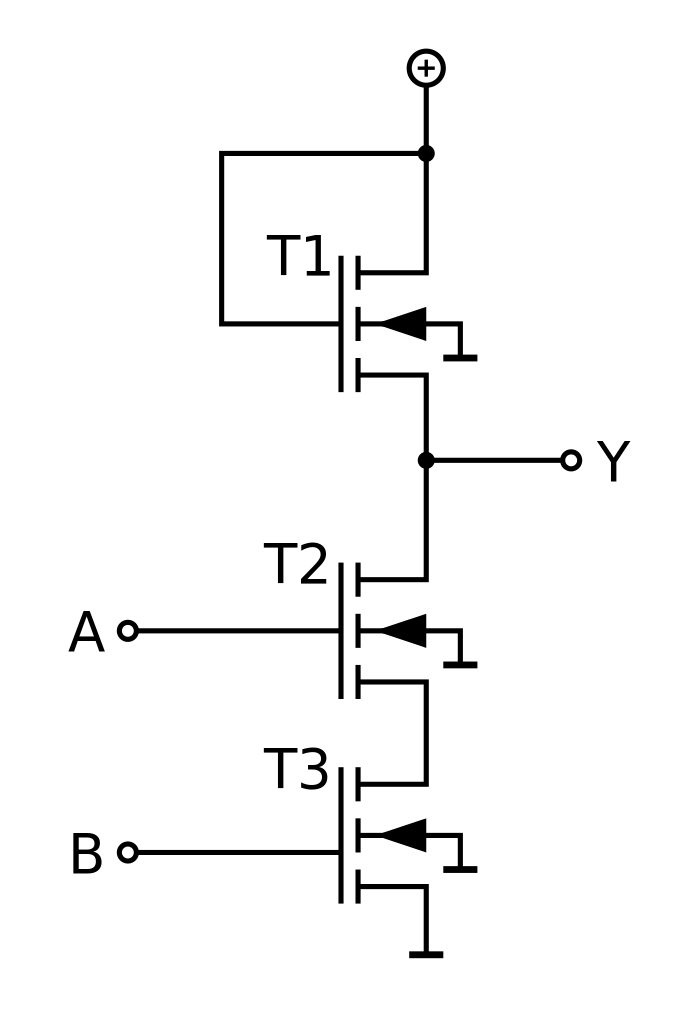
\includegraphics{./img/nmos-nand}
\\
Sannhetstabellen blir lik NAND i forige seksjon.
Når både A og B er på vil transistoren lede.
Når transistoren leder vil Y bringes ned til jord AKA null.



\paragraph{NOR} \mbox \\
NOR port implementert med NMOS.
\\
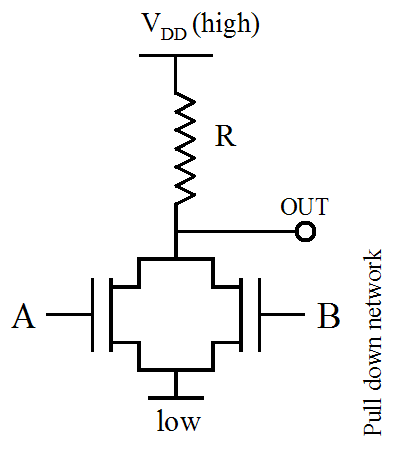
\includegraphics{./img/nmos-nor}
\\
På bildet kan man bytte ut R med en nmos-motstand (gate og drain koblet).

Hvis minst én av A eller B er på, vil transistoren lede.
Når en eller begge transistorene leder, bringes Y til jord.


  \subsubsection{DTL}
    TODO: tegn og forklar en DTL-NAND (se skrivebok)


  \subsubsection{TTL}
    TODO


\subsection{Kombinatoriske kretser}
  Vi skiller mellom kombinatoriske og sekvensielle kretser.
Noen operasjoner, som pluss og minus, er uavhengig av hva som har skjedd før.
Kombinasjonen av tall A pluss tall B gir en sum.

Ved en if-statement, if(var == 22), må man hente variable fra minne og ta en
beslutning basert på hva den variabelen var satt til.
Logikken er altså avhengig av hva som har skjedd tidligere.
Dette er sekvensiell logikk.

I denne subseksjonen skal vi se på kombinatorisk logikk hvor f.eks. summen
av to tall er uavhengig av tidligere hendelser.


  \subsubsection{Binær addisjon}
    Dette er lett å søke opp på internett.


  \subsubsection{Adders}
    TODO


\subsection{Sekvensielle kretser}
    sekvensiell TODO


  \subsubsection{Dekoder / Enkoder}
    \paragraph{Dekoder} \mbox{} \\
TODO



\paragraph{Enkoder} \mbox{} \\
TODO


  \subsubsection{ROM}
    rom TODO


  \subsubsection{Latches}
    latches n flip-flops TODO



\paragraph{SR-latch} \mbox{} \\
TODO



\paragraph{Synkron SR-latch} \mbox{} \\
TODO



\paragraph{D-latch} \mbox{} \\
TODO


  \section{Uke 11 - Flip-flops og operasjonsforsterkere}
    Kap. 22, s 752 -787

\subsection{Flip-flopper}
  Hva er forksjellen på en flip-flip og en latch?
Ordene \emph{har} vært brukt mye om hverandre, men det har blitt enighet
om forskjellen.
En flip-flop er en klokkestyrt latch.
En latch styres ikke av en klokke.
Men bjørn i sinn at ordene fremdeles brukes om hverandre.

  \subsubsection{JK flip-flop}
    I en vanlig SR flip-flop er oppførselen uspesifisert for to høye input.
JK flip-flop løser problemet ved å bestemme at to høye input betyr flip.
Hva enn som var på output blir motsatt av hva det var.
\begin{figure}[H]
  \caption{JK flip-flop}
  \centering
    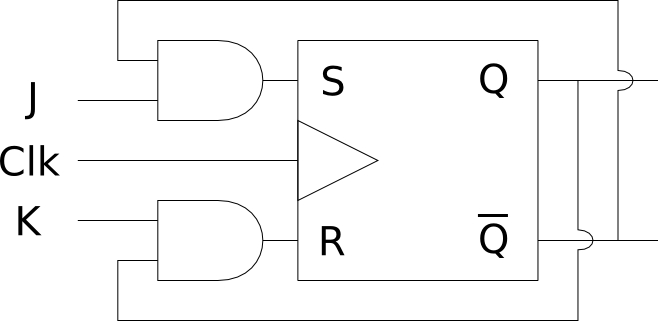
\includegraphics[width=\textwidth]{./img/jk}
\end{figure}
Sannhetstabellen til en JK flip-flop ser ut som følgende.
\begin{table}[H]
  \caption{JK sannhetstabell}
  \centering
  \begin{tabular}{c|c|c|c}
    J & K & Q & $\overline{Q}$ \\ \hline
    0 & 0 & Q & $\overline{Q}$ \\
    1 & 0 & 1 & 0 \\
    0 & 1 & 0 & 1 \\
    1 & 1 & $\overline{Q}$ & Q
  \end{tabular}
\end{table}

  \subsubsection{Master/Slave flip-flop}
    En master/slave flip-flop lages ved å koble to flip-flops i serie, hvor den
siste av dem mottar det inverterte klokkesignalet til den første.
Den bakerste flip-flopen endres kun når den første gjør det.
Derfor er den første master og den andre slave.
\begin{figure}[H]
  \caption{Master/slave flip-flop}
  \centering
  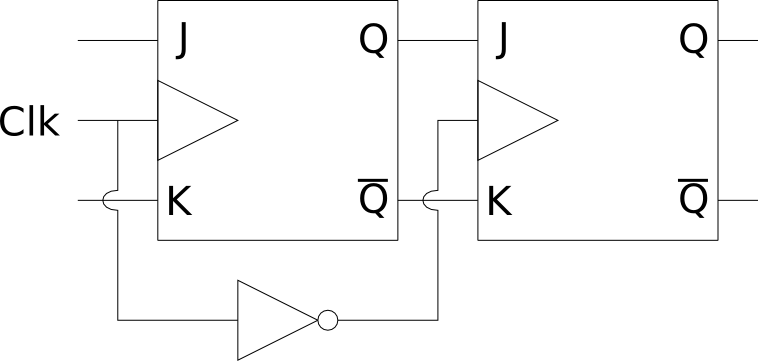
\includegraphics[width=\textwidth]{./img/master-slave}
\end{figure}

  \subsubsection{Binære tellere}
    Binære tellere gir et binært tall på output som øker med én for hver gang
inngangsklokken tikker.
\\\\
Ved å bruke master/slave flip-flops koblet i serie hvor Q er koblet til neste
sin klokke.
Alle inngangene, J og Q, er satt til høy, slik at hver gang klokka tikke endres
Q og $\overline{Q}$ til det motsatte.
\begin{figure}[H]
  \caption{4bit binærteller.}
  \centering
  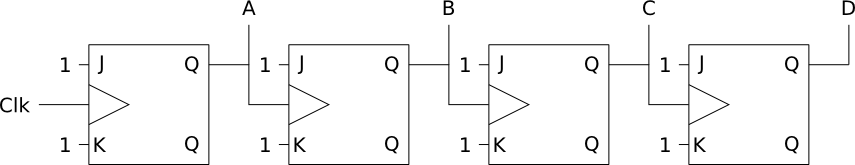
\includegraphics[width=\textwidth]{./img/biteller}
\end{figure}
Output A, B, C og D er little endian.
Det vil si at den minst betydningsfulle biten kommer først.
Dvs $A=2^0$, $B=2^1$ osv.
\\\\
Når klokka tikker, veksler A fra av og på.
Når A tikker, veksler B fra av og på, osv.
Resultatet blir en teller.
\begin{figure}[H]
  \caption{Binærteller output}
  \centering
  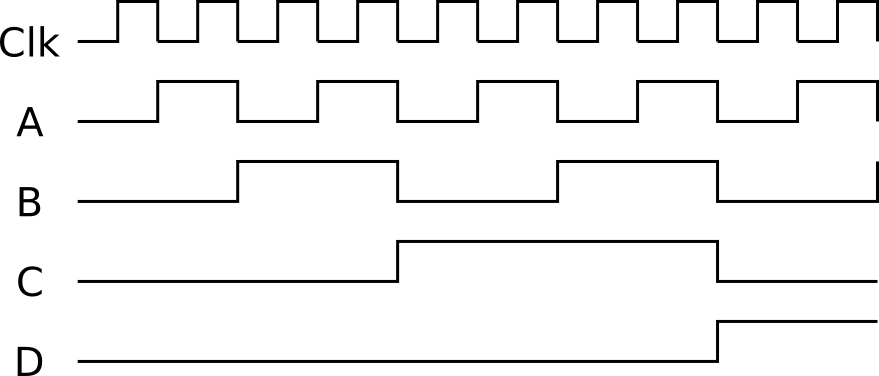
\includegraphics[width=\textwidth]{./img/biteller-output}
\end{figure}
Hvis du ser på output ser du at den teller oppover 0000, 1000, 0100, 1100 osv.

  \subsubsection{Dekadeteller}
    TODO

  \subsubsection{Registere}
    TODO


\subsection{Op-amp}
  \subsubsection{Integrated Circuits}
    TODO

  \subsubsection{Op-amp}
    En opamp er en spennings forsterker som bl.a. kan brukes til analoge
regneoperasjoner.
\\\\
Egenskaper:
\begin{itemize}
\item Veldig høy forsterkning: $10^5$ til $10^6$.
\item Høy inngangsmotstand gjør den effektiv.
\item Stabil i forhold til temperatur.
\item Kontrollert fasegang.
\item Differansekobling på inngangen.
\end{itemize}

\begin{figure}[H]
  \caption{Symbol for en op-amp.}
  \centering
  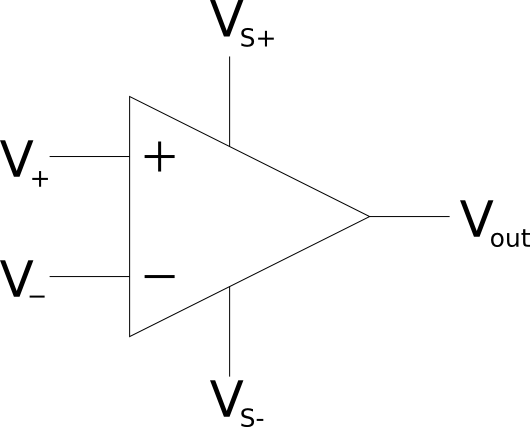
\includegraphics[width=0.5\textwidth]{./img/opamp-symbol}
\end{figure}



\paragraph{LM741} \mbox{} \\
Et eksempel på en IC implementasjon av en opamp er LM741.
\begin{figure}[H]
  \caption{LM741 pinout}
  \centering
  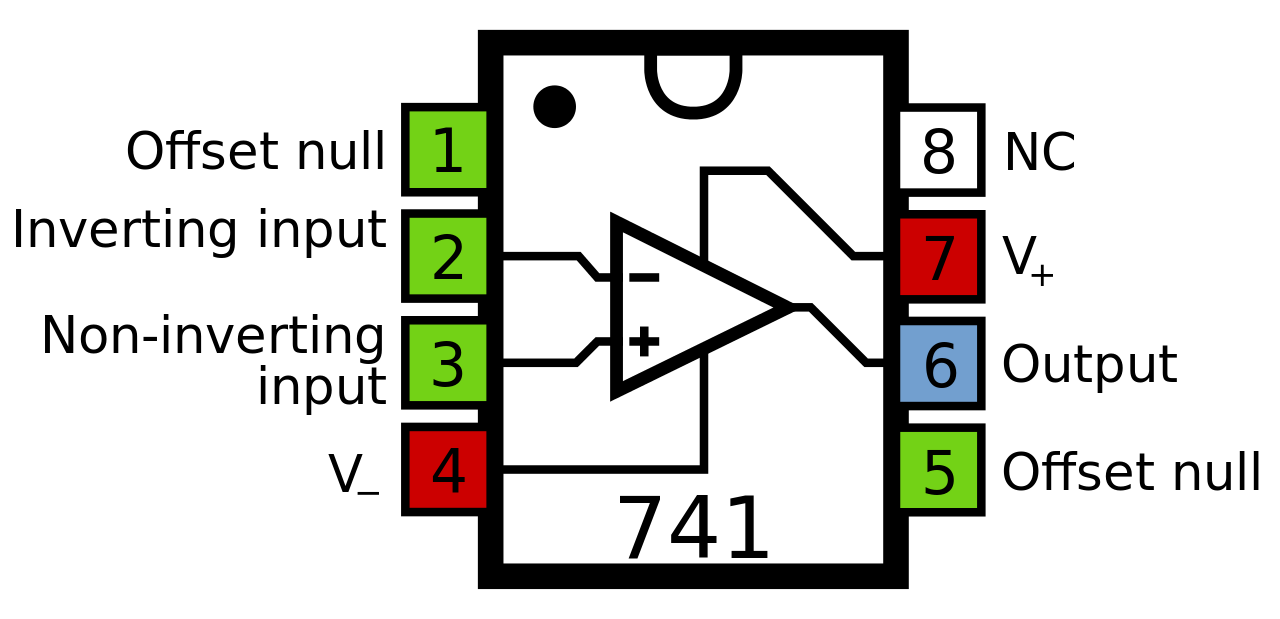
\includegraphics[width=0.5\textwidth]{./img/lm741}
\end{figure}

  \subsubsection{Tre viktige parametre}
    \begin{description}
\item [$R_i$] Indre motstand: $R_i > \SI{1}{M\ohm}$
\item [$A_v$] Forsterkning: $A_v > 10^5$
\item [$R_o$] Utgangsmotstand: $R_o < \SI{100}{\ohm}$
\end{description}



TODO

  \subsubsection{Inverterende Forsterker}
    TODO


  \section{Uke 12}
    \subsection{Påskeferie}
  Ingen forelesning denne uka.

  \section{Uke 13}
    \subsection{Påskeferie}
  Ingen forelesning denne uka.

  \section{Uke 14 - Anvendelse av OpAmp}
    Kap. 23, s.798 -836

Vi fortsetter der Uke11 slapp, med operasjonsforsterkere.

\subsection{Kretser med OpAmp}
  \subsubsection{Ikke-inverterende forsterker}
    TODO
  \subsubsection{Integratorkobling}
    TODO
  \subsubsection{Addisjon med OpAmp}
    TODO
  \subsubsection{Differensial forsterker}
    TODO
  \subsubsection{Eksponential forsterker}
    TODO
  \subsubsection{Logaritmisk forsterker}
    TODO
\subsection{Egenskaper ved OpAmper}
  \subsubsection{Virtuelt nullpunkt}
    TODO
  \subsubsection{Parametre for OpAmper}
    TODO
  \subsubsection{Gain BandWidth Product}
    TODO

  \section{Uke 15 - Aktive Frekvensfiltre m/OpAmper}
    Kap. 23, s.798 -836

\subsection{Enheter}
  \subsubsection{Slew Rate}
    Slew rate er et mål på en krets evne til å reagere på endringer i spenning.
Spesifikasjonen til f.eks. en opamp kan garantere en viss slew rate sånn at man
kan beregne om den er brukbar i en gitt krets.
Signalet gitt på input skal kunne gjenskapes perfekt (med en hvis toleranse)
på output.

Slew rate (S) er gitt som forholdet mellom spenning/sekund.
$$S \geq \frac{dv}{dt}$$

I en forsterker må følgende tilfredsstilles
$$S \geq 2 \cdot \pi \cdot f \cdot V_{pk}$$

  \subsubsection{Common-mode Rejection Ratio}
    En opamp skal helst forsterke forskjellen mellom input A og B, men som vi vet
er aldri elektroniske komponenter ideelle.

I en ideell opamp er utgangsspenningen $v_o = A_v(v_+ - v_-)$.
En ideell opamp skulle avvise et signal som ankommer begge input.

Common-mode Rejection Ratio er gitt ved
$$CMRR = \frac{A_v (differensiell)}{A_v (common-mode)}$$

\subsection{Aktive Frekvensfiltre med Operasjonsforsterkere}
  Det finnes mange typer filtre og de kan deles inn etter måten de er bygd opp på
eller hvordan de former signaler.
Vi har: aktive og passive filtre, bredbånd- og smalbåndfiltre,
høypass, lavpass, båndpass, båndstopp, notch...

TODO consider illustations (4 hovedtyper).

  \subsubsection{Parametre}
    \paragraph{} \mbox{Båndbredde} \\
Ved filtre som båndpass og båndstopp er båndbredden gitt fra grensefrekvensene.
Fra $V_{pk}$ til en reduksjon på -3dB finner man grensefrekvensene.
Båndbredden er avstanden mellom disse frekvensene.
$$BW = f_{c2} - f_{c1}$$



\paragraph{} \mbox{Q-Verdi} \\
Q-Verdien sier noe om hvor bratt et filter avtar.
En høy Q betyr brattere filter.

Q-Verdien er gitt ved den geometriske senterfrekvensen $f_0$.
$f_0$ er nesten som gjennomsnitt, men tar høyde for logaritmisk skala.
$$f_0 = \sqrt{f_{c1} \cdot f_{c2}}$$

Q-Verdien er forholdet mellom senterfrekvensen og båndbredden.
$$Q = \frac{f_0}{BW}$$



\paragraph{} \mbox{Pol} \\
Når vi lager filtre med opamper bruker vi RC kretser.
En pol er én RC krets.
Det vil bli mer tydelig i seksjonen med implementasjonseksempler.



\paragraph{} \mbox{Orden} \\
Antall poler i et filter avgjør filterets orden.
Det bestemmer også hvor fort signalet avtar.

1. Ordens filter
Har én pol.
Avtar med 20dB per dekade.

2. Ordens filter
Har to poler.
Avtar med 40dB per dekade.

3. Ordens filter
Har tre poler.
Avtar med 60dB per dekade.
osv...

  \subsubsection{Typer}
    Vi skal se på tre typer filtre: Butterworth, Bessel og Chebyshev.
De forskjellige typene har forksjellige egenskaper som velges etter
hvilke egenskaper som passer formålet.

\begin{figure}[H]
  \caption{Filtertyper}
  \centering
  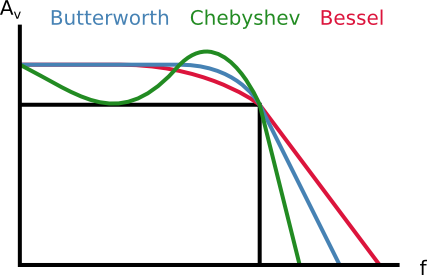
\includegraphics[width=0.67\textwidth]{./img/filtertyper}
\end{figure}

\paragraph{Butterorth (Maximally flat)} \mbox{} \\
+ Flat respons $A_v$ relativt konstant innenfor båndet). \\
+ Mest brukte aktive filteret. \\
- Fasegang endres når filteret avtar.

\paragraph{Bessel} \mbox{} \\
+ Konstant fasegang. \\
+ HiFi (High Fidelity).

\paragraph{Chebyshev} \mbox{} \\
+ Bratt rolloff. \\
- Ikke konstant spenningsforsterkning.

\subsection{Implementasjoner}
  \subsubsection{Lavpass (Butterworth)}
    TODO variabel/unity
  \subsubsection{Lavpass (Butterworth 2. orden)}
    TODO
  \subsubsection{Høypass (Butterworth)}
    TODO
  \subsubsection{Høypass (Butterworth 2. orden)}
    TODO
  \subsubsection{Båndpass (Kombinerer høypass/lavpass)}
    TODO
  \subsubsection{Notch/Båndstopp}
    Et notchfilter er et spesialtilfelle av båndstop hvor Q-Verdien er veldig høy.
Signalet sender til både et lavpass- og et høypassfilter før de legges sammen
i en adder som plusser sammen signalene.

\begin{figure}[H]
  \caption{Skjematikk for notch filter}
  \centering
  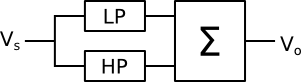
\includegraphics[width=0.67\textwidth]{./img/notch-kobling}
\end{figure}

Den resulterende formen på signalet blir

\begin{figure}[H]
  \caption{Notch filter frekvens og forsterkning}
  \centering
  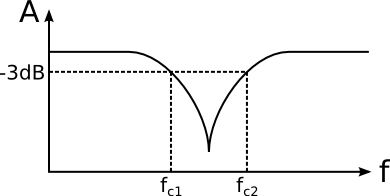
\includegraphics[width=0.67\textwidth]{./img/notch-frekvens}
\end{figure}

\subsection{Tilbakekobling (feedback)}
  Feedback oppstår når output fra et system kobles tilbake på systemets input.
Det brukes til: Linearisering, stabilisering og regulering og kontroll.
Vi tegner det på følgende måte:

\begin{figure}[H]
  \caption{Negativ feedback}
  \centering
  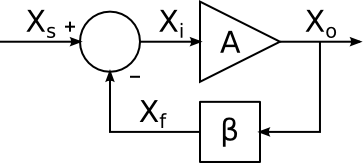
\includegraphics[width=0.67\textwidth]{./img/negfeedback}
\end{figure}

$$X_s = \text{signal inn}$$
$$X_o = \text{signal ut}$$
$$X_i = \text{signal til OpAmp}$$
$$X_f = \text{feedbacksignal}$$

Disse verdiene er gitt ved
$$X_i = X_s - \beta \cdot X_o$$
$$X_o = A \cdot (X_s - \beta \cdot X_o)
      = \frac{A \cdot X_s}{1 + A \cdot \beta}$$
$$A_f = \frac{X_o}{X_s} = \frac{A}{1 + A \cdot \beta}$$

Ved positiv feedback har vi
$$A_f = \frac{X_o}{X_s} = \frac{A}{1 - A \cdot \beta}$$


  \section{Uke 16 - Feedback, Millereffekt, Oscillatorer}
    Kap. 23, s. 798 -836

\subsection{Feedback}
  Fortsetter fra forrige kapittel.

Avhengig av forholdet mellom $A \cdot \beta$ vil signalet endre seg
på forskjellig måte.

\paragraph{Loopgain $< 1$} \mbox{} \\
\begin{figure}[H]
  \caption{Oscillasjon dør ut}
  \centering
  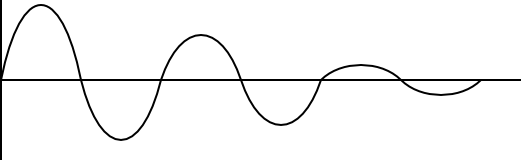
\includegraphics[width=0.5\textwidth]{./img/fadingsignal}
\end{figure}

\paragraph{Loopgain $> 1$} \mbox{} \\
\begin{figure}[H]
  \caption{Signalet øker til clipping}
  \centering
  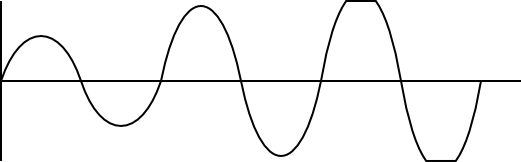
\includegraphics[width=0.5\textwidth]{./img/gainingsignal}
\end{figure}

\paragraph{Loopgain $= 1$} \mbox{} \\
\begin{figure}[H]
  \caption{Stabilt signal}
  \centering
  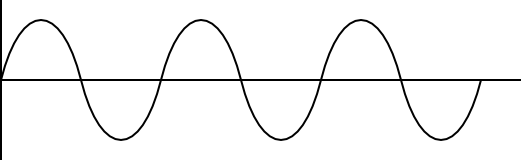
\includegraphics[width=0.5\textwidth]{./img/stabiltsignal}
\end{figure}

\subsection{Millereffekt}
  Miller effekt oppstår når man kobler en kondensator i feedbackloopen på en
inverterende opamp.

Kondensatorens reaktans er gitt ved:
$$X_C = \frac{1}{j\omega C} = \frac{1}{2\pi fC}$$

\begin{figure}[H]
  \caption{Kondensator i feedbackloopen}
  \centering
  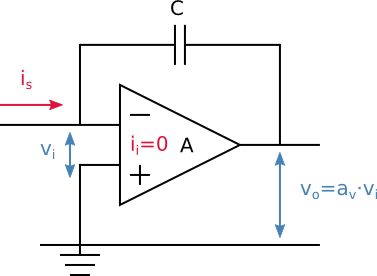
\includegraphics[width=0.5\textwidth]{./img/miller}
\end{figure}

Kondensatoren virker som om den er (1+A) ganger større enn den er.
$$i_s = \frac{v_i\cdot X_C}{v_i + A\cdot v_i}
      = \frac{X_C}{1 + A}
      = \frac{1}{j\omega C(1+A)}$$

Det gir 'millerkapasitet' $C_M$ lik:
$$C_M = C(1+A)$$

Dette betyr at høye frekvenser kuttes tidligere:
$$f_h = \frac{1}{2\pi \cdot R_{inn} \cdot C(1+A)}$$

\begin{figure}[H]
  \caption{Miller-cutoff vs vanlig cutoff}
  \centering
  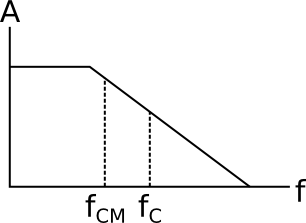
\includegraphics[width=0.5\textwidth]{./img/millercutoff}
\end{figure}

\subsection{Oscillatorer}
  En oscillator lager et periodisk svingende signal.
I musikalsk anvendelse kan dette være grunnlag for en synthesizer eller effect.
I elektronikk kan signalet fungere som en klokke for synkroniserte kretser.

Vi skal se på fire ulike typer: \\
Faseskift-oscillator \\
Wien brigde-oscillatorer \\
Avstemte oscillatorer \\
Krystall-oscillatorer

  \subsubsection{Faseskift-oscillatorer}
    Faseskift-oscillatoren produserer en sinusbølge.
Fordi faseforskyvningen avhenger av frekvens regnes den som ustabil og
er lite brukt.
Den har ingen input-signal, men trigges av en impuls.

De er sammensatt av et nettverk av RC-kretser.
For å kompansere for tapet over disse må loopgain være 1.
$$A_f = \frac{A}{1 - A\cdot \beta}$$
$$A\cdot \beta \to 1
  \implies A_f \to \infty$$

\begin{circuitikz} \draw
(8,1.5) node[op amp] (opamp) {}
(opamp.+) node[left] {}
(opamp.-) node[left] {}
(opamp.out) node[right] {}

%Resistors
(0,0) node[ground] {} -- (6,0)
(1,0) to[R] (1,2)
(3,0) to[R] (3,2)
(5,0) to[R] (5,2)
(6,0) -- (6,1)
      -- (opamp.+)

%Capasitors
(opamp.-) -- (5,2)
      to[C] (3,2)
      to[C] (1,2)
      to[C] (-1,2)
      -- (-1, 3)
      -- (9.5,3)
      -- (9.5,1.5)

%Output
(opamp.out) -- (10.5,1.5)
      node[label=$V_o$] {}
      ;
\end{circuitikz}

Opampen inverterer signalet 180 grader,
mens RC-leddene inverterer det ytterligere 180 for en gitt frekvens.
Frekvensen den oscillerer med er gitt ved:
$$f = \frac{1}{2\pi RC\sqrt{6}}$$

  \subsubsection{Wien brigde-oscillatorer}
    Stabil og en av de mest brukte RC-oscillatorene.
Den bruker både positiv og negativ feedback.

\resizebox{\textwidth}{!}{
\begin{circuitikz} \draw
(4.5,4.5) node[op amp] (opamp) {}
(opamp.+) node[left] {}
(opamp.-) node[left] {}
(opamp.out) node[right] {}
(0,4) node[ground] {}
      -- (0,5)
      to[R, l=$R_5$] (2,5)
      to[short, *-] (opamp.-)

%Negativ
(2,5) -- (2,7)
      to[R, l=$R_4$, -*] (7,7)
      to[short, -*] (9,7)
      -- (11,7)
(7,4.5) to[short, -*] (9,4.5)
      to[short, -*] (11,4.5)
      to[short, -o] (12,4.5)
      node[label=$V_{out}$] {}
(7,7) to[R, l=$R_3$] (7,4.5)
(9,4.5) to[D, l=$D_1$, mirror] (9,7)
(11,7) to[D, l=$D_2$] (11,4.5)

%Positiv
(1,0) node[ground] {}
      to[C, l=$C_1$] (1,2)
      to[short, -*] (3,2)
      -- (3,4)
      -- (opamp.+)
(3,0) node[ground] {}
      to[R, l=$R_1$] (3,2)
      to[C, l=$C_2$] (5,2)
      to[R, l=$R_2$] (7,2)
      to[short, -*] (7,4.5)
      -- (opamp.out)
      ;
\end{circuitikz}
} %resizebox




\paragraph{Positiv} \mbox{} \\
Den positive tilbakekoblingen kontrollerer svingningene.

\begin{figure}[H]
  \caption{Resonansfrekvens}
  \centering
  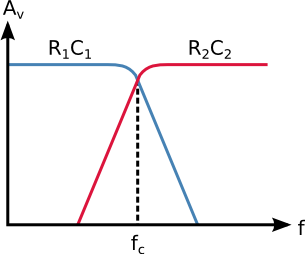
\includegraphics[width=0.5\textwidth]{./img/wien}
\end{figure}

$$R_1 = R_2$$
$$C_1 = C_2$$
$$f_c = \frac{1}{2\pi RC}$$



\paragraph{Negativ} \mbox{} \\
Den negative tilbakekoblingen kontrollerer closed loop gain $A_{CL}$.
Feedback loopen gir en forsterkning, men diodene begrenser spenningen.
$$A_{CL} = \frac{R_f}{R_{inn}} + 1
         = \frac{R_3 + R_4}{R_5} + 1$$

\begin{figure}[H]
  \caption{Diodene clipper signalet ved stor forsterkning}
  \centering
  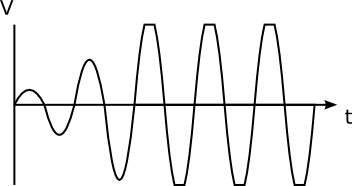
\includegraphics[width=0.5\textwidth]{./img/wienclipp}
\end{figure}

  \subsubsection{Avstemte oscillatorer}
    Avstemte oscillatorer er veldig presise, men også veldig dyre og lite brukt.

De er bygd opp av en inverterende forsterker og LC-ledd (spole og kondensator).

Av de flere typene som finnes er de mest vanlige: \\
Colpitts \\
Hartley

  \subsubsection{Krystall-oscillatorer}
    Krystall-oscillatorer er teknologien bak mange klokker og mesteparten av
teknologien vi bruker i dag.
De fungerer ved piezoelektrisk effekt.
Det vil si at strøm påført elementet medfører mekanisk deformasjon.
Tilsvarende vil et mekanisk trykk på elementet generere elektrisk spenning.
Resonansfrekvensen bestemmes av krystallets fysiske størrelse.

Fordeler:
\begin{itemize}
  \item Stabil
  \item Høy frekvens
  \item Billig
  \item Lavt energikrav
\end{itemize}

\begin{circuitikz} \draw
%Bottom
(1,0) to[short, o-] (1,1)
(0,1) -- (2,1)

%Left
(0,1) to[R, l=$R$] (0,3)
      to[C, l=$C$] (0,5)
      to[L, l=$L$] (0,7)

%Right
(2,7) to[C, l=$C_m$] (2,1)

%Top
(0,7) -- (2,7)
(1,7) to[short, -o] (1,8)
      ;
\end{circuitikz}

Krystallet har to resonansfrekvenser avhengig av om man ser på serieresonansen
av $RCL$ eller parallellresosansen med $RL$ og $C_M$.

\begin{figure}[H]
  \caption{Resonansfrekvens for paralell og serie}
  \centering
  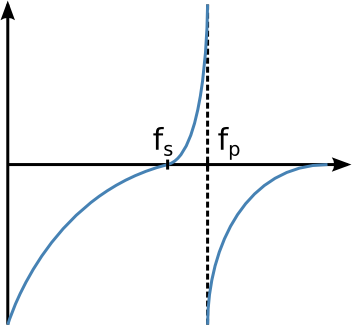
\includegraphics[width=0.5\textwidth]{./img/krystallresonans}
\end{figure}


  \section{Uke 17 - Signalbehandling}
    Kap. 24, s. 845-871

\subsection{Spenningsforskjell}
  \subsubsection{Komparator}
    En komparator tar inn et signal og sammenligner det med en referansespenning.

\begin{circuitikz} \draw
(4.5,4.5) node[op amp] (opamp) {}
(opamp.+) node[left] {signal}
(opamp.-) node[left] {ref}
(opamp.out) node[right] {ut}
      ;
\end{circuitikz}

Den gir utslag (0 eller 1) når signalet overstiger referansen.

\begin{figure}[H]
  \centering
  \caption{Komparator indikerer overstigelse av referanse}
  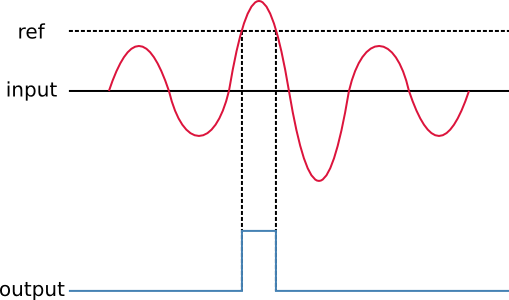
\includegraphics[width=0.67\textwidth]{./img/komparator}
\end{figure}

  \subsubsection{Shmitt-trigger}
    \input{./tex/uke17/shmitt}
\subsection{Digital/Analog}
  \subsubsection{R-2R}
    Med et trappesystem av motstander kan man konvertere et binært digitalt input
til et analogt output.

Q1 er den minst signifikante bit (LSB).

\begin{circuitikz} \draw
(0,2) node[ground] {}
      to[R, l=$2R$] (2,2)
      to[R, l=$R$] (4,2)
      to[R, l=$R$] (6,2)
      to[R, l=$R$] (8,2)
      -- (8,4)
      to[short, l=$V_{out}$, -o] (10,4)
(2,0) node[anchor=north] {Q1}
      to[R, l=$2R$, -*] (2,2)
(4,0) node[anchor=north] {Q2}
      to[R, l=$2R$, -*] (4,2)
(6,0) node[anchor=north] {Q3}
      to[R, l=$2R$, -*] (6,2)
(8,0) node[anchor=north] {Q4}
      to[R, l=$2R$, -*] (8,2)
      to[R, l=$2R$] (10,2)
      node[ground] {}
      ;
\end{circuitikz}

$$V_{ut} = \frac{V_1}{16} + \frac{V_2}{8} + \frac{V_3}{4} + \frac{V_4}{2}$$

  \subsubsection{OpAmp Addisjon}
    Se seksjon 14.4.
\subsection{Analog/Digital}
  \subsubsection{Samplingsteorem}
    For å konvertere et analogt signal til digitalt, leser man av spenningen
ved diskrete intervaller.
Hvor hyppig disse avlesningene forekommer kalles sample rate.

For å kunne gjengi en brukbar digital representasjon av signalet, må vi ha
en høy nok sample rate.
Sample raten bør være minst dobbelt så høy som den høyeste frekvensen
man sampler.
Den høyeste frekvensen mennesker kan høre er 20kHz, så CD-er har en sample rate
på 44.1kHz.
Jo flere punkter man sampler (høy sample rate), jo bedre blir recordingen.

\begin{itemize}
\item Hørbart: 20Hz - 20kHz
\item CD: 44.1kHz
\item Lydkort: 48kHz
\item Pro-lydkort: 96kHz - 192kHz
\end{itemize}

\begin{figure}[H]
  \centering
  \caption{Forskjellig sample rate}
  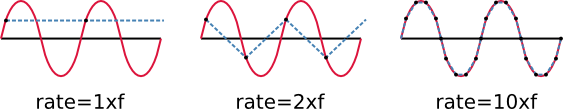
\includegraphics[width=\textwidth]{./img/samplerate}
\end{figure}

  \subsubsection{Sample-Hold}
    For å kunne lese av en spenningsverdi når vi sampler, må vi kunne låse fast
signalet så det ikke endrer seg under avlesning.
Da bruker man en sample-hold.

\begin{circuitikz} \draw
%OpAmp 1
(2,2) node[op amp, yscale=-1] (opamp) {}
(opamp.+) node[left] {Vinn}
(opamp.-) node[left] {}
(opamp.out) node[right] {}
(opamp.out) -- (3.5,2)
      -- (3.5,0.5)
      -- (0,0.5)
      -- (0,1.5)
      -- (opamp.-)

%Fet
(5,2) node[pjfet, rotate=90] (pjfet) {}
(pjfet.G) node[anchor=north] {}
(pjfet.D) node[anchor=west] {}
(pjfet.S) node[anchor=east] {}
      (3.5,2) -- (pjfet.S)
      (pjfet.G) -- (4.75,0)
      -- (4,0)
      node[anchor=north] {Gate kontroll}

%Capasitor
(pjfet.D) -- (7,2)
      to[C] (7,0)
      node[ground] {}

%OpAmp 2
(10,1.5) node[op amp, yscale=-1] (opamp) {}
(opamp.+) node[] {}
(opamp.-) node[] {}
(opamp.out) node[] {}
(opamp.out) -- (11.5,1.5)
      -- (11.5,0)
      -- (8,0)
      -- (8,1)
      -- (opamp.-)
(7,2) -- (opamp.+)
(opamp.out) to[short, -o, l=$V_{out}$] (12.5,1.5)
      ;
\end{circuitikz}

  \subsubsection{Counting A/D}
    En counting ADC bruker en binærteller for å \emph{'nærme seg'} riktig verdi.
Binærtelleren tikker høyere og høyere helt til komperatoren bekrefter at
man har funnet høy nok verdi.

En klokke brukes for å samkjøre det hele.

\marginpar{Endianness: Om vi leser binære tall fra høyre eller venstre}
\marginpar{MSB: Most significant byte}
\marginpar{LSB: Least significant byte}

\begin{figure}[H]
  \centering
  \caption{}
  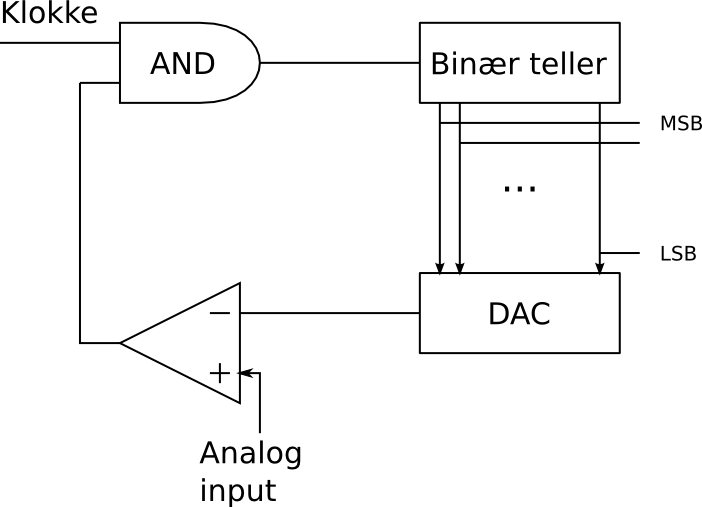
\includegraphics[width=0.67\textwidth]{./img/countingADC}
\end{figure}

For en verdi låst med Sample-Hold tikker klokka opp til riktig verdi.

\begin{figure}[H]
  \centering
  \caption{Output fra counting ADC}
  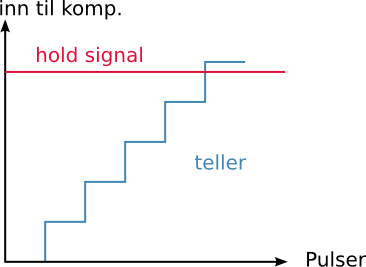
\includegraphics[width=0.5\textwidth]{./img/countingout}
\end{figure}

Skal man lese n-bit trenger konverteringen $2^n$ klokkepulser.

  \subsubsection{Successive Approximation A/D}
    Successive approximation ADC, eller tilnærmings ADC, fungerer nesten som
en counting ADC.

Den teller nærmere og nærmere et hold signal, men den tikker ikke gradvis
opp fra bunnen.
Den veksler frem og tilbake rundt signalet og nærmer seg gradvis.

\begin{figure}[H]
  \centering
  \caption{ADC som tilnærmer seg signalet}
  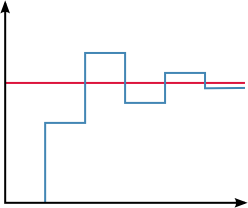
\includegraphics[width=0.5\textwidth]{./img/oppnedout}
\end{figure}

\begin{figure}[H]
  \centering
  \caption{Successive approximation ADC}
  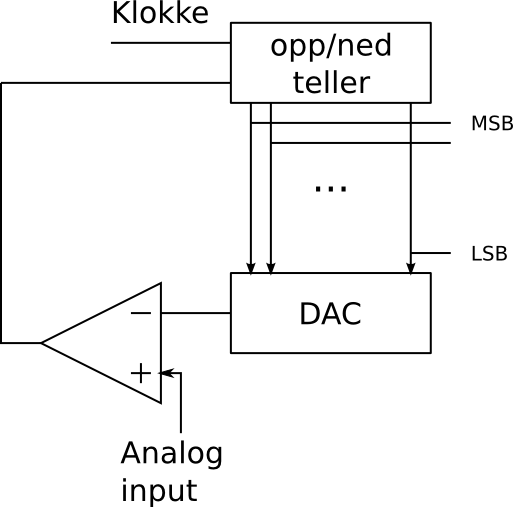
\includegraphics[width=0.5\textwidth]{./img/oppnedADC}
\end{figure}

  \subsubsection{Flash konverter}
    Flash konverteren er veldig rask, men også veldig dyr.

Signalet føres til mange komperatorer samtidig, hvor hver komperator er
forhåndsinnstilt til en referansespenning.
Den oversetter momentant fra digital til analog.

\begin{figure}[H]
  \centering
  \caption{Flash converter / Flash ADC}
  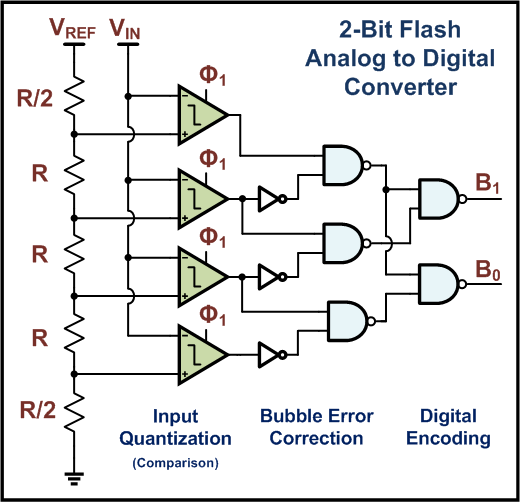
\includegraphics[width=0.67\textwidth]{./img/flashadc}
\end{figure}

En 2bit flash ADC trenger 4 komparatorer.
Likeledes trenger en 8bit flash ADC $2^8 = 256$ komparatorer.


  \section{Uke 18 - Signalbehandling fortsatt}
    \subsection{Sampling}
  \subsubsection{Begreper}
    \paragraph{Oppløsning} \mbox{} \\
Når man konverterer fra et analogt signal til et digitalt blir signalet
representert binært.
Oppløsningen, eller bit-dybden, er hvor mange bit vi bruker på å representere
signalet.

Med bare 2-bit får man et grovt, forstyrret signal.
Jo høyere bit depth jo mer presis blir samplingen.
8-bit gir 256 nivåer (255 hvis like mange bit skal fordeles over og under null).



\paragraph{Konverteringstid} \mbox{} \\
I de ADCene vi så på tar det tid for klokka å tikke nærmere signalets verdi.
Tiden det tar for én slik sampling kalles konverteringstid.



\paragraph{Kvantiseringsfeil} \mbox{} \\
Når vi leser av et signal fra Sample-Hold, vil det opprinelige signalet ha
forandret seg i mellomtiden.
Med dette oppstår det som kalles kvantiseringsfeil.
Med høyere oppløsning vil dette reduserer, men da vil konverteringstiden øke.

  \subsubsection{Delta-sigma konverter}
    I en $\Delta \Sigma$ DAC blir det analoge signalet integrert og oversatt
til en 1-bit strøm.

\begin{figure}[H]
  \centering
  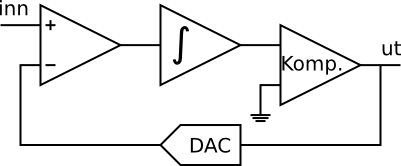
\includegraphics[width = 0.5\textwidth]{./img/deltasigma}
  \caption{Delta-sigma ADC}
\end{figure}

\subsection{Multivibratorer}
  Multivibratorer brukes til å lage pulser som f.eks. kan brukes i en timer.

  \subsubsection{Astabil}
    Denne kretsen har ingen input og veksler på egenhånd mellom to tilstander.

\begin{figure}[H]
  \centering
  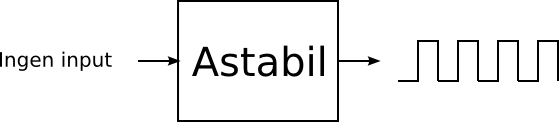
\includegraphics[width=0.5\textwidth]{./img/astabil}
  \caption{Astabil multivibrator}
\end{figure}

  \subsubsection{Monostabil}
    Denne kretsen trigges av en input impuls og vil etter en gitt tid dø ut.
Kretsen har \emph{én} stabil tilstand.

\begin{figure}[H]
  \centering
  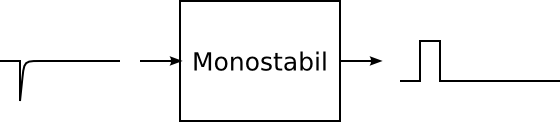
\includegraphics[width=0.5\textwidth]{./img/monostabil}
  \caption{Monostabil multivibrator}
\end{figure}

  \subsubsection{Bistabil}
    En bistabil latch eller flip-flop kan skrus av og på.

\begin{figure}[H]
  \centering
  \includegraphics[width=0.5\textwidth]{./img/bistabil}
  \caption{Bistabil multivibrator}
\end{figure}

\subsection{Sensorer}
  \subsubsection{Definisjon}
    En sensor er noe som spesifiserer en tilstand.
Begrepet dekker enkle sensorer som f.eks. en temperatursensor, men også
sammensatte sensorer som ABS systemet på en bil.
Den reagerer på et bestemt fenomen og gir et signal ut.

En sensor må være:
\begin{itemize}
  \item Følsom for bestemt fenomen.
  \item Ufølsom for andre fenomener.
  \item Må ikke selv lage forstyrrelser i fenomenet.
\end{itemize}

  \subsubsection{Presisjon vs nøyaktighet}
    Når vi spesifiserer egenskapene til en sensor skiller vi mellom presisjon
og nøyaktighet.

Presisjon sier hvor stor spredning det er.
Høy presisjon betyr liten spredning.

Nøyaktighet sier hvor nærme målet man er.
Stor nøyaktighet kan ha mye variasjon, men variasjonene er sentrert rundt
det riktige området.

\begin{figure}[H]
  \centering
  \includegraphics[width=0.67\textwidth]{./img/presisjon}
  \caption{Presisjon vs Nøyaktighet}
\end{figure}

Nøyaktighet kan sies å representere systemavvik og
presisjon tilfeldighet.

\begin{figure}[H]
  \centering
  \includegraphics[width=0.33\textwidth]{./img/avvik}
  \caption{Presisjon/nøyaktighet grafert}
\end{figure}


  \section{Uke 19 - Spenningsregulator og Radio}
    Kap. 25, s 881-895

\subsection{Spenningsregulator}
  I en powersupply (se seksjon 6.5) kjøres et AC signal gjennom en likeretter,
et filter og en regulator.
Vi skal se på hvordan slike spennings-regulatorer er bygget opp.

Hvis man skal kjøpe en IC med spenningsregulator finnes det hovedsaklig
fire typer:\\
Fixed positiv: Gir en bestemt positiv spenning.\\
Fixed negativ: Gir en bestemt negativ spenning.\\
Justerbar: Man kan velge mellom bestemte intervaller.\\
Dual-Tracking: Gir en bestemt spenning både som negativ og positiv.

  \subsubsection{Serie-regulator}
    Serieregulatorer har en eller flere enheter plassert i serie med lasten.

\begin{figure}[H]
  \centering
  \includegraphics[width=0.67\textwidth]{./img/serie-boks}
  \caption{Regulatoren er i serie med lasten}
\end{figure}

En implementasjon av en serieregulator er en pass transistor regulator.

\begin{circuitikz} \draw
(4,3) node[npn,rotate=90] (npn) {}
(npn.base)

(0,3) node[label=$V_{inn}$] {}
      to[short, o-] (3.3,3)
(2,3) -- (2,2)
      to[R] (4,2)
      -- (4,2.2)

(4,0) node[ground] {}
      to[zD*] (4,2)

(4.7,3) node[label=$V_{ut}$] {}
      to[R, l=$R_L$, o-] (7,3)
      -- (7,2.5)
      node[ground] {}
      ;
\end{circuitikz}

Spenningsfall over $V_{BE}$ gjør at ledningsevnen til transistoren øker
og en relativt stabil spennings opprettholdes.

Merk! Denne kretsen har hverken feilbehandling eller sikring.

  \subsubsection{Shunt-regularor (parallell)}
    \begin{figure}[H]
  \centering
  \includegraphics[width=0.67\textwidth]{./img/parallell-boks}
  \caption{Regulatoren er i parallell med lasten}
\end{figure}

Beklager, jeg orker ikke tegne opp en implementasjon.

\subsection{Radio}
  \subsubsection{Amplitude-modulasjon}
    I amplitudemodulasjon har man det opprinnelige signalet man vil overføre,
og en carrier wave som skal \emph{bære} signalet.

Input-signalet flyttes slik at det ikke har noen negativ komponent,
deretter multipliseres det med carrier bølgen.

Resultatet er et signal med høyere frekvens hvor amplituden gir formen
til det opprinnelige signalet.

\begin{figure}[H]
  \centering
  \includegraphics[width=0.67\textwidth]{./img/am}
  \caption{Input multipliseres med carrier wave}
\end{figure}

  \subsubsection{Frekvens-modulasjon}
    I frequency modulation, FM, vil bærebølgen endre frekvens bestemt av
input signalet.
Når input har høy amplitude får output høyere frekvens.
Når input har lav amplitude blir det lavere frekvens.

\begin{figure}[H]
  \centering
  \includegraphics[width=0.67\textwidth]{./img/fm}
  \caption{Output frekvens er raskere der amplituden er høy}
\end{figure}



\paragraph{Problem med stereo} \mbox{} \\
Gamle mottakere var kun kompatible med mono, så når stereo skulle implementeres
i fm ble det problematisk.

Mono-signalet inneholder lyd for høyre og venstre kombinert (L+R).

Løsningen var å bruke en annen kanal til å sende (L-R).
På denne måten kan gamle radioer bruke (L+R), men moderne radioer kan anvende
matematikk på signalene for å hente ut stereo signalene hver for seg.
$$(L+R)+(L-R)=2L$$
$$(L+R)-(L-R)=2R$$

For å sende dette over bare én frekvens brukes tidsmultipleksing (TDM).
Senderen veksler mellom å sende annen hvert signal.
Hvis man veksler med en frekvens på 38kHz kan man reprodusere 15kHz signaler
hos mottaker.

  \subsubsection{Faseskift-modulasjon}
    Phase shift keying (PSK), faseskift modulering, brukes for å sende
digitale signaler.

En firkantpuls kommer inn på input, dette kombineres med en bærebølge.
Der hvor input skifter fra lav til høy, eller motsatt, får bærebølgen en
faseforskyvning på 180 grader.

\begin{figure}[H]
  \centering
  \includegraphics[width=0.67\textwidth]{./img/psk}
  \caption{Faseskift i overgang mellom lav/høy}
\end{figure}

Denne teknologien brukes i bl.a. WiFi, bluetooth og RFID.


  \section{Uke 20}
    \subsection{Eksamensøving}
      Tid for å øve til eksamen.
  \section{Uke 21}
    \subsection{Eksamensøving}
      Tid for å øve til eksamen.
  \section{Uke 22}
    \subsection{Eksamensøving}
      Tid for å øve til eksamen.
  \section{Uke 23}
    \subsection{Eksamensøving}
      Tid for å øve til eksamen.
\end{document}
